%-----------------------------------------------------------------------------
%
%               Template for sigplanconf LaTeX Class
%
% Name:         sigplanconf-template.tex
%
% Purpose:      A template for sigplanconf.cls, which is a LaTeX 2e class
%               file for SIGPLAN conference proceedings.
%
% Guide:        Refer to "Author's Guide to the ACM SIGPLAN Class,"
%               sigplanconf-guide.pdf
%
% Author:       Paul C. Anagnostopoulos
%               Windfall Software
%               978 371-2316
%               paul@windfall.com
%
% Created:      15 February 2005
%
%-----------------------------------------------------------------------------


\documentclass[preprint]{sigplanconf}

% The following \documentclass options may be useful:

% preprint      Remove this option only once the paper is in final form.
% 10pt          To set in 10-point type instead of 9-point.
% 11pt          To set in 11-point type instead of 9-point.
% authoryear    To obtain author/year citation style instead of numeric.

\usepackage{amsmath}
\usepackage{hyperref}
\usepackage{graphicx}


\begin{document}

\special{papersize=8.5in,11in}
\setlength{\pdfpageheight}{\paperheight}
\setlength{\pdfpagewidth}{\paperwidth}

\conferenceinfo{CONF 'yy}{Month d--d, 20yy, City, ST, Country} 
\copyrightyear{20yy} 
\copyrightdata{978-1-nnnn-nnnn-n/yy/mm} 
\doi{nnnnnnn.nnnnnnn}

% Uncomment one of the following two, if you are not going for the 
% traditional copyright transfer agreement.

%\exclusivelicense                % ACM gets exclusive license to publish, 
                                  % you retain copyright

%\permissiontopublish             % ACM gets nonexclusive license to publish
                                  % (paid open-access papers, 
                                  % short abstracts)

\titlebanner{Member Num: 9574664; Advisor: Ruzica Piskac; Cat: Graduate; }        % These are ignored unless
\preprintfooter{short description of paper}   % 'preprint' option specified.

\title{Javascript as an Intermediate Language for FRP}
%\subtitle{Subtitle Text, if any}

\authorinfo{Mark Santolucito}
           {Yale University - 51 Prospect St., New Haven, CT 06511}
           {mark.santolucito@yale.edu}

\maketitle

\section{Introduction}

%probelm
Functional Reactive Programming (FRP) is an exciting and popular way to make interactive applications in a functional style.
However, creating production level applications with FRP remains prohibitively difficult, especially for mobile platforms.
Each mobile platform only supports particular languages and architectures, so many cross-compiling tools must be installed and managed.
While many users are able to write FRP applications, the lack of deployment options has limited mobile FRP apps to only the most dedicated FRP researchers.

We propose using Javascript as an intermediate language to eliminate most of the technical hurdles to publishing applications written with FRP, allowing more programmers to use FRP in production.
We have developed a tool that automatically creates a mobile app package.
It works for any any mobile platform and takes an Elm program as input, though other languages like Haskell could also be supported.
The user can develop exclusively in the FRP language, use a foreign function interface (FFI) to interface with lower level languages and hardware, or use FRP for only isolated pieces of the app.

%motivation

\section{Background}
Although deployment is difficult, development of interactive apps can be faster and easier using FRP.
One particular strength is that prototypes can be generated very quickly, and these prototypes are easily extended to full applications.
This has been used in many interactive multimedia applications such as music, robotics, and games\cite{euterpea,robots,yampa}.
As an example, see Figure ~\ref{fig:easy} for a very short drawing application written in Elm.
To write this in another style would be very verbose and likely difficult.

%why FRP for mobile dev, why is it so good
%example code in picture
\begin{figure*}
  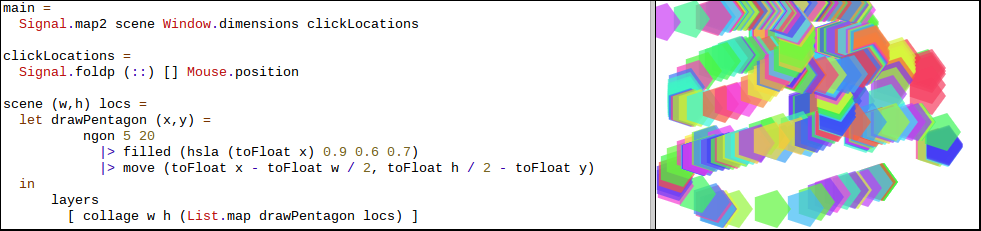
\includegraphics[width=\textwidth,height=4cm]{easy.png}
  \caption{Easy code for a drawing app that traces the mouse (or finger for a touch screen) with colored shapes.}
  \label{fig:easy}
\end{figure*}

%related/motivation
FRP implementations include many libraries in Haskell, the dedicated FRP language Elm, and the Sodium project which ports FRP to more language like Java and C\cite{euterpea,elm,sodium}.
FRP research is most developed for functional languages like Haskell and Elm, but each mobile platform requires device specific languages (e.g Java for Android).
Ideally, FRP programs could be cross-compiled to the target platform without significant interference in the development process.


%reduce this section
A GHC cross-compiler exists for Apple's iOS platform that could possibly provide a way to use a Haskell FRP library to develop iOS apps.
Perez, in work with Keera Studios, has successfully cross-compiled Haskell to Android and published the game \textit{Magic Cookies}\cite{cookies}.
Although promising, the source code for this remains closed source and the setup has been difficult to reproduce due to many installation steps.
Windows phone development remains largely unexplored.
These however require that all tool chains be installed and managed separately - a large cost for an average user.

\section{Results}
%soltn
To simplify the process, we compile FRP programs to an intermediate language, then use a \textit{platform agnostic} tool to compile the intermediate language to any target device desired.
The intermediate language presented here is Javascript and platform agnostic tool is Phonegap.
For Haskell, ghcjs can compile program to Javascript, while Elm is compiled to Javascript by default\cite{ghcjs}.
Phonegap allows users to create apps for any platforms by writing Javascript\cite{phonegap}. 
We instead send the generated (and incomprehensible) Javascript to Phonegap to create a package for any mobile device.
Here Javascript is functioning as an intermediate language - the user does not need to look at it for the system to work.

%APIs
Mobile development also relies on the use of APIs.
Many platform specific APIs have similar Javascript implementation, which can be used via the FRP languages FFI.
For APIs that require native code, Phonegap provides textit{plugins} as a foreign function interface (FFI) from Javascript to the lower level language.
The Javascript plugin code can then be accessed via the FRP language through that FFI.
Both ghcjs and Elm provide a Javascript FFI to enable this chain. 

%Performance
Performance is a concern when using an intermediate language without optimizations. 
Preliminary testing shows optimizations are not needed for simple game development using this tool. 
A common measure for performance in FRP systems is the frames per second (fps) that can be displayed.
Any number above 32 fps is generally acceptable, and our proof of concept app maintains $>$150 fps on a Nexus 5 running Android 5.1.1.
However, this is only for a 2D game, so performance measures for more complex systems will be needed in future work.

Our demo app uses FRP to read the touch interface native to the mobile hardware and control a simple game.
The app also uses a plugin FFI to show native ads, mixing Javascript code with Elm.
The source code and app files are available at \url{github.com/santolucito/elm_games}.

This approach is unique because it treats the high-level language of one tool as an intermediate language for another. 
It is unique in its simplicity because it leverages Phonegap to unify the work flow for all platforms - iOS, Android and Windows apps are all created from the same system.
There is no need to install a different cross-compiler for each target device.
This approach also works well in practice, providing good performance and access to low-level APIs when needed.
 
The development of FRP and functional languages in general relies on adoption by industry.
Simplifying the work flow to bring FRP code to market will encourage future work in FRP.

% We recommend abbrvnat bibliography style.

\bibliographystyle{abbrvnat}

% The bibliography should be embedded for final submission.

%\begin{thebibliography}{}
%\softraggedright
%\bibitem[Smith et~al.(2009)Hudak, Paul]{euterpeaii}
%\end{thebibliography}

\bibliography{ICFP}

\end{document}

%                       Revision History
%                       -------- -------
%  Date         Person  Ver.    Change
%  ----         ------  ----    ------

%  2013.06.29   TU      0.1--4  comments on permission/copyright notices

